	\section{Schaltverluste, Kühlung}
B2C als Beispiel:\\\\
in einem ersten Schritt muss der Strom durch den Thyristor berechnet werden:\\
\begin{tabular}{ll}
  Spitzenwert des Thyristorstromes&\ $I_{Rm} = \frac{U_{2m}}{R}$\\\\
  Mittelwert des Thyristorstromes &\ $I_{T AV} = \frac{1}{2\pi}\int\limits_{\alpha}^{\pi}I_{Rm} \cdot sin(\beta) \cdot d\beta, \beta = \omega t$\\
  &\ $I_{T AV} = \frac{I_{Rm}}{2\pi} \cdot (1+cos\alpha)$\\\\
  Effektivwert des Thyristorstromes &\ $I_{T RMS} = \sqrt{\frac{I_{RM}^2}{2\pi}\int\limits_{\alpha}^{\pi}sin^2(\beta)d\beta}$\\
  &\ $I_{T RMS} = \frac{I_{Rm}}{2}\sqrt{\frac{\pi - \alpha}{\pi}+\frac{sin2\alpha}{2\pi}}$\\\\
\end{tabular}

\begin{figure}[htbp]
  \begin{minipage}[t]{6cm}
    \vspace{0pt}
    \centering
    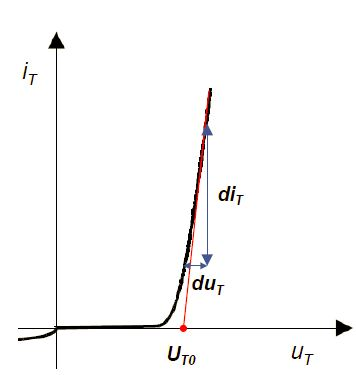
\includegraphics[width = 5cm]{./pictures/kennlinieThyristor} 
  \end{minipage}
  \hfill
  \begin{minipage}[t]{6cm}
    \vspace{0pt}
    Durchlassrichtung: $i_{T}, u_{T}$\\
    Schwellenspannung: $U_{T0}$\\
    Differentieller Durchlasswiderstand: $r_{T} = \dfrac{du_{T}}{di_{T}}$\\
    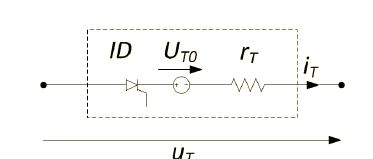
\includegraphics[width = 4cm]{./pictures/schemaThyristor}\\
    $u_{T} = U_{T0}+i_{T}(t) \cdot r_{T}$
  \end{minipage}
\end{figure}

momentane Verlustleistung: $p(t) = u_{T}(t) \cdot i_{T}(t)$\\
\begin{tabular}{ll}
  Mittelwert der Verlustleistung: &\ $P_{T} = \frac{1}{T}\int\limits_{0}^{T}u_{T}(t) \cdot i_{T}(t) \cdot dt$\\
  &\ $P_{T} = U_{T0} \cdot \frac{1}{T}\int\limits_{0}^{T}i_{T}(t)dt+r_{T} \cdot \frac{1}{T}\int\limits_{0}^{T}i_{T}^2(t)dt$\\\\
  &\ $P_{T} = U_{T0} \cdot I_{T AV} + r_{T} \cdot I_{T RMS}^2$\\
  &\ $I_{T AV}$ ist der Mittelwert und $I_{T RMS}$ der\\ &\ Effektivwert des Thyristorstroms\\
\end{tabular}

\textbf{Der Wert für $U_{T0}$ kann aus dem Datenblatt des Thyristors herausgelesen werden.}\\\\\\
\begin{tabular}{|l|l|}
  \hline
  \textbf{Thermische Kenngrössen} &\ \textbf{Elektrische Kenngrössen}\\
  \hline
  Wärmeleistung $ P (W) $ &\ Strom $ I (A) $\\
  \hline
  Temperaturunterschied $\vartheta (K)$ &\ Spannung $U (V)$\\
  \hline
  Wärmewiderstand $R_{th} (\frac{K}{W})$ &\ Widerstand $R (\frac{V}{A})$\\
  \hline
\end{tabular}

\subsection{Thyristor ohne Kühlkörper}
\begin{figure}[htbp]
  \begin{minipage}[t]{6cm}
    \vspace{0pt}
    \centering
    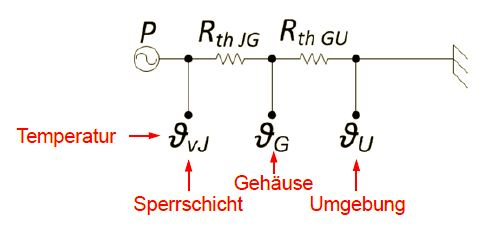
\includegraphics[width = 5cm]{./pictures/ohneKuehlkoerper} 
  \end{minipage}
  \hfill
  \begin{minipage}[t]{6cm}
    \vspace{0pt}
    $\vartheta_{vJ} - \vartheta_{U} = P \cdot (R_{th JG}+ R_{th GU})$\\
    $ \vartheta_{vj} = P \cdot (R_{th JG}+ R_{th GU}) + \vartheta_{U}$\\\\\\
    \textbf{$R_{th}$ muss wiederum aus dem Datenblatt herausgelesen werden.}
  \end{minipage}
\end{figure}

\subsection{Thyristor mit Kühlkörper}
\begin{figure}[htbp]
  \begin{minipage}[t]{6cm}
    \vspace{0pt}
    \centering
    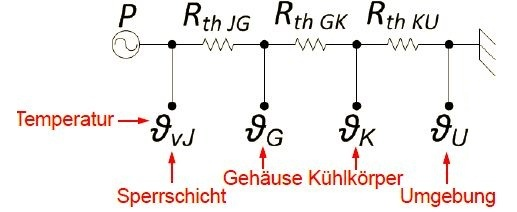
\includegraphics[width = 5cm]{./pictures/mitKuehlkoerper} 
  \end{minipage}
  \hfill
  \begin{minipage}[t]{6cm}
    \vspace{0pt}
    $\vartheta_{vJ} - \vartheta_{U} = P \cdot (R_{th JG}+ R_{th GK}+ R_{th KU})$\\
    $ \vartheta_{vj} = P \cdot (R_{th JG}+ R_{th Gk} +R_{th KU}) + \vartheta_{U}$\\\\\\
    
  \end{minipage}
\end{figure}
